\section*{Exploring the Red Sequence of AGN with the {\it James Webb Space Telescope}}

\smallskip
\smallskip
\noindent
Things We Know About AGN/Quasars::
\begin{itemize}
\item Blue Quasars are in enhanced distrubed systems at $z\sim0.7$ (Villforth et al.)
\item ``Red'' quasars generally merger at $z\sim2.5$ (Glikman et al. 2016), but ``red'' here is a somewhat red+radio definition...
\item Peak of optical QLF at $z\sim2-3$ (Richards et al. 2006; Ross et al. 2014)
\item There is a trend of radio fraction in QSOs with $(g-i)$ colour; the redder the colour, the larger 
the radio fraction (Klindt et al. 2018)
\end{itemize}


\smallskip
\smallskip
\noindent
Things We {\it don't} Know About AGN/Quasars::
\begin{itemize}
\item The host properties of SDSS/BOSS $z=2-3$ QSOs
\item Is there a {\it range} in red quasar host properites??
\item Is there a {\it ``transition colour''} above which mergers are enhanced?
\item Is there a {\it transitional Radio Loudness} above which mergers are enhanced?
\end{itemize}


\smallskip
\smallskip
\noindent
{\bf General Idea::} \\
NIRCam Imaging, and/or NIRSpec spectroscopy (Long Slit? IFU?) of a sample of ``red'' to ``extremely red'' quasars. \\
\begin{itemize}
\item What are the host galaxy morphologies of Red Quasars? 
\item Are ``Red'' quasars more distrubed than ``Extremely Red'' quasars?
\item Are red radio-loud quasars in different hosts than red radio-quiet quasars??
\item Are the narrow lines offset from the broadlines in the red quasars?
\item {\it What physical properties (SFR, morphology disturbanace, radio fraction, outflow etc.) change along the
AGN Red Sequence??}
\end{itemize}


\smallskip
\smallskip
\noindent
{\bf General Sample::} \\
X-Shooter Red Quasar Sample (Radio Loud? Radio Quiet? TBD...)\\
``Core'' ERQs from Hamann et al. (2017). $i$-W3 selected, with \civ EW selection too. \\
Select the subset of ``core'' ERQs that are still $r$-W4 objects...??\\
``Hot DOGs'' (aka W1W2-drops)\\


\smallskip
\smallskip
\noindent
Questions to answer/things to address:: 
\begin{itemize}
\item Why not {\it HST}??  Want to go redder than e.g. F160W	($H$-Short at 1.545$\mu$m, FWHM=0.29$\mu$m
\item Why not {\it ALMA}?? Will/can use ALMA for e.g. SFRs instead of MIRI.
\end{itemize}


\smallskip
\smallskip
\noindent
``Cool Ideas....'' 
\begin{itemize}
\item Hopkins (2008) Figure 1, for real, for the Red objects, at $z\approx2.5$. 
\end{itemize}

\hspace{-7.5cm}
\begin{figure}[h]
  \begin{center}
    \hspace{-0.5cm}
%    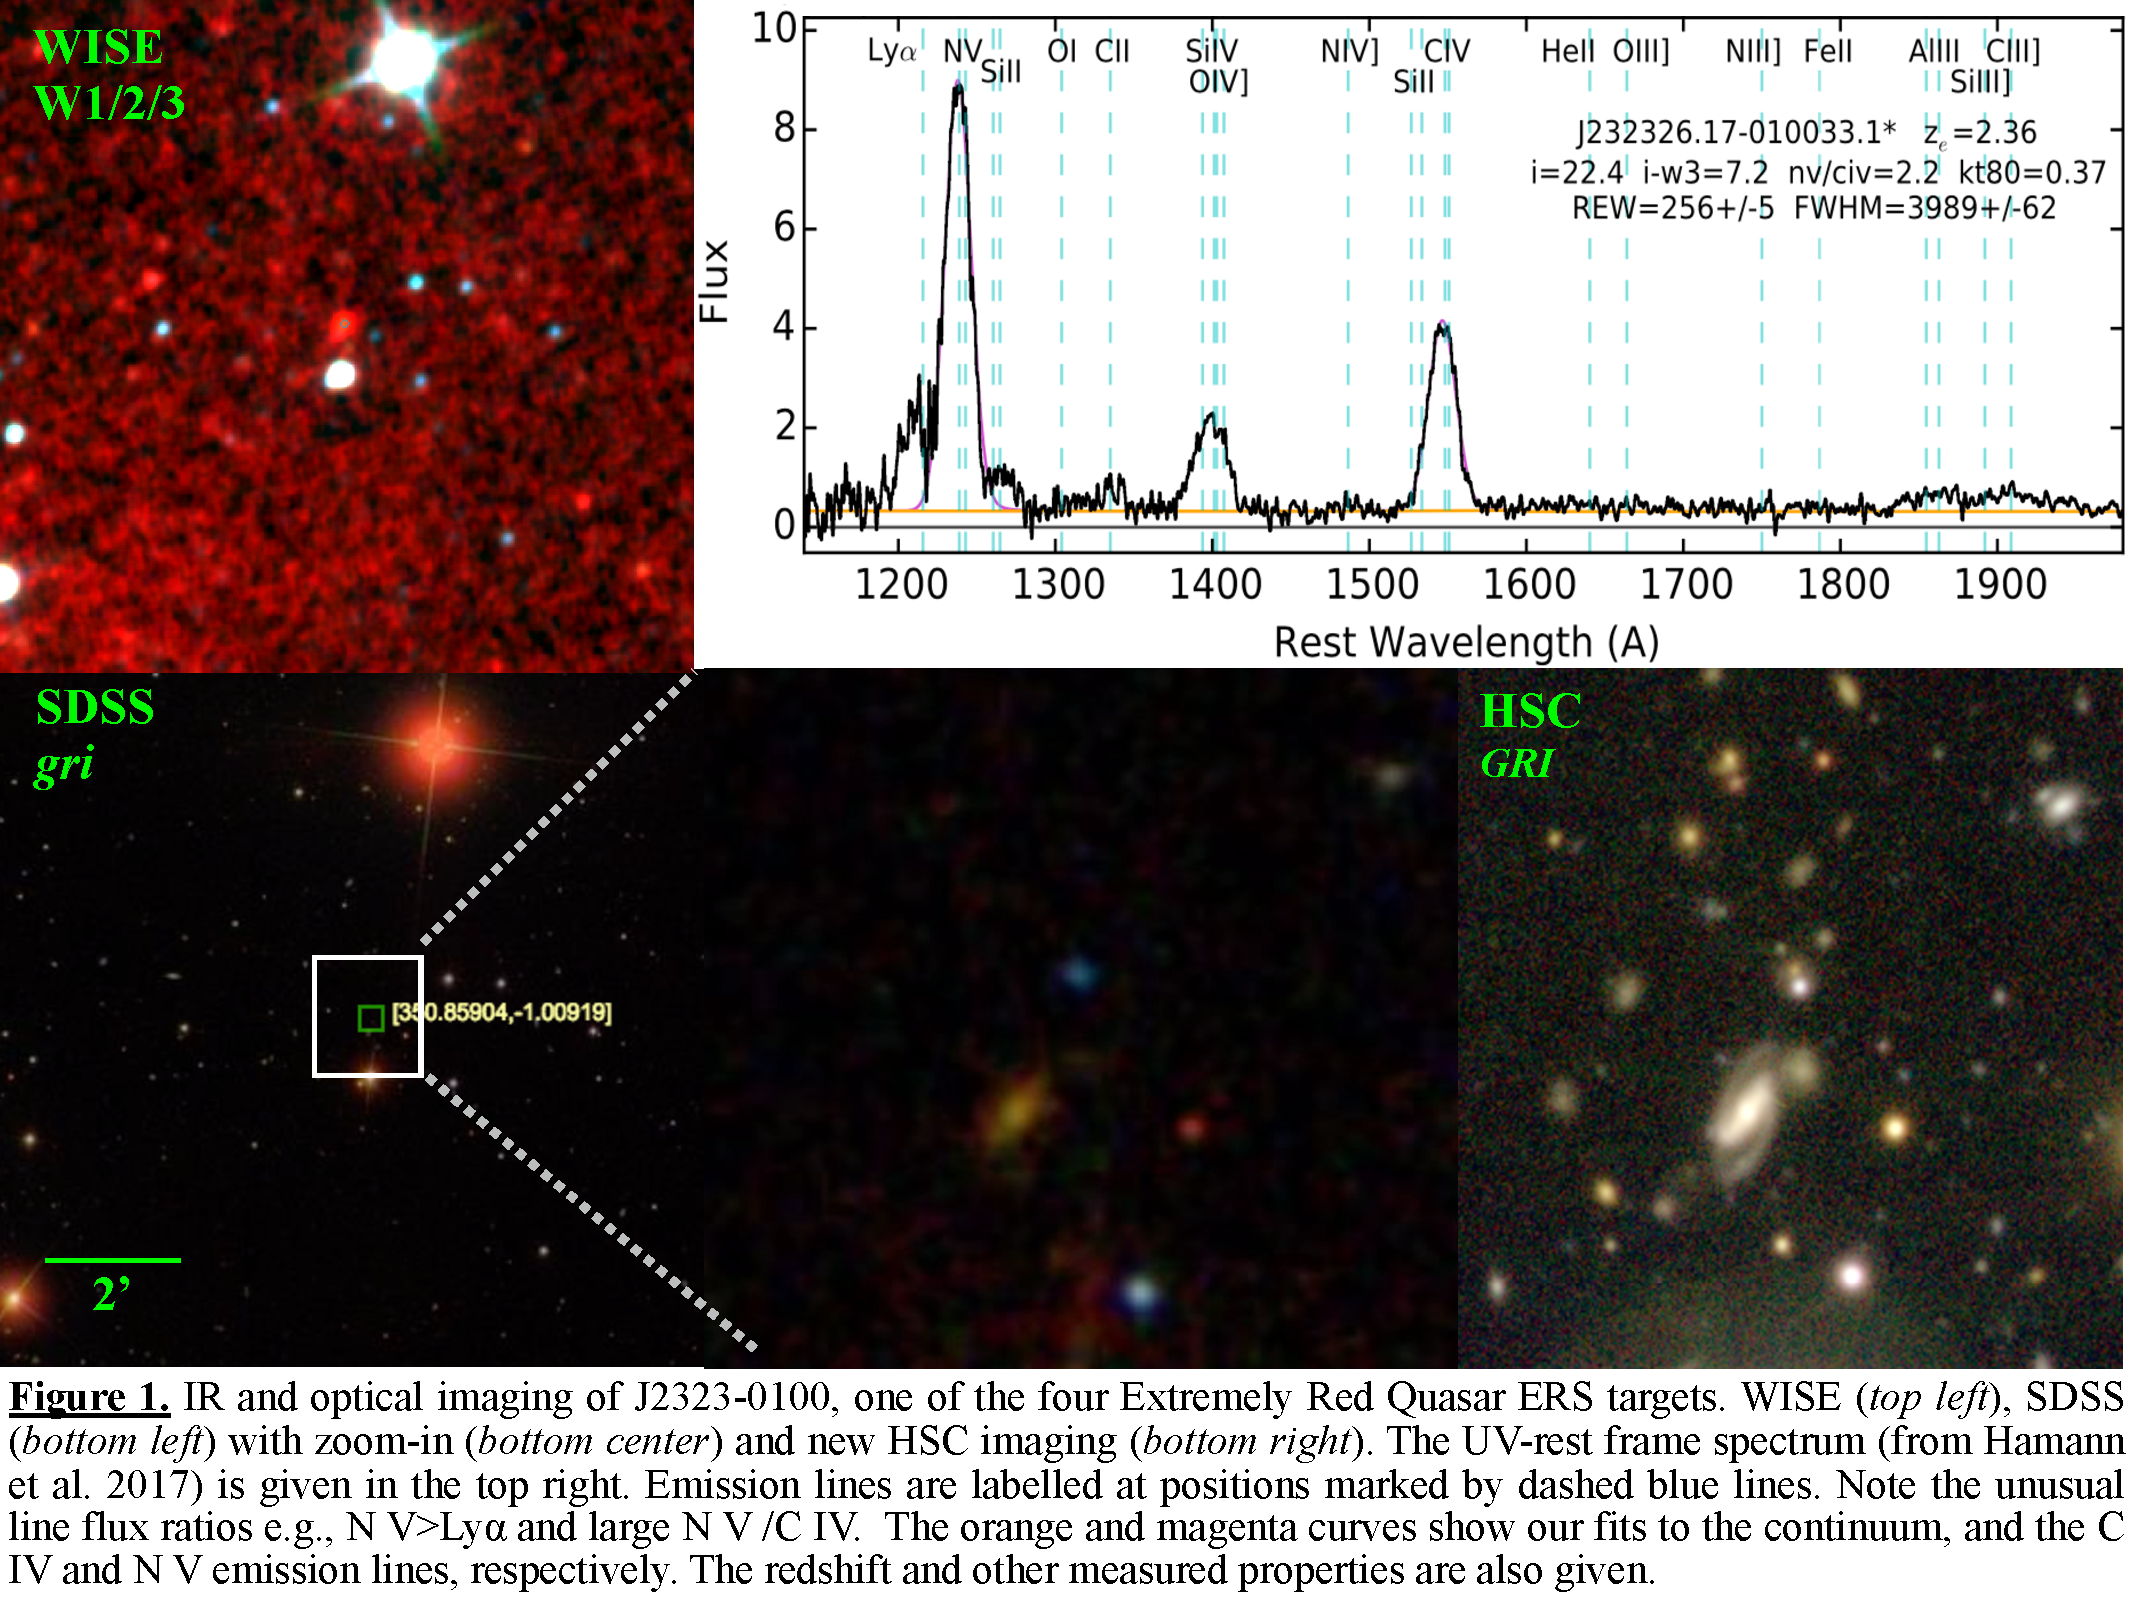
\includegraphics[]{WISE_SDSSzoomHSC_ERQ-image_v2.pdf}
    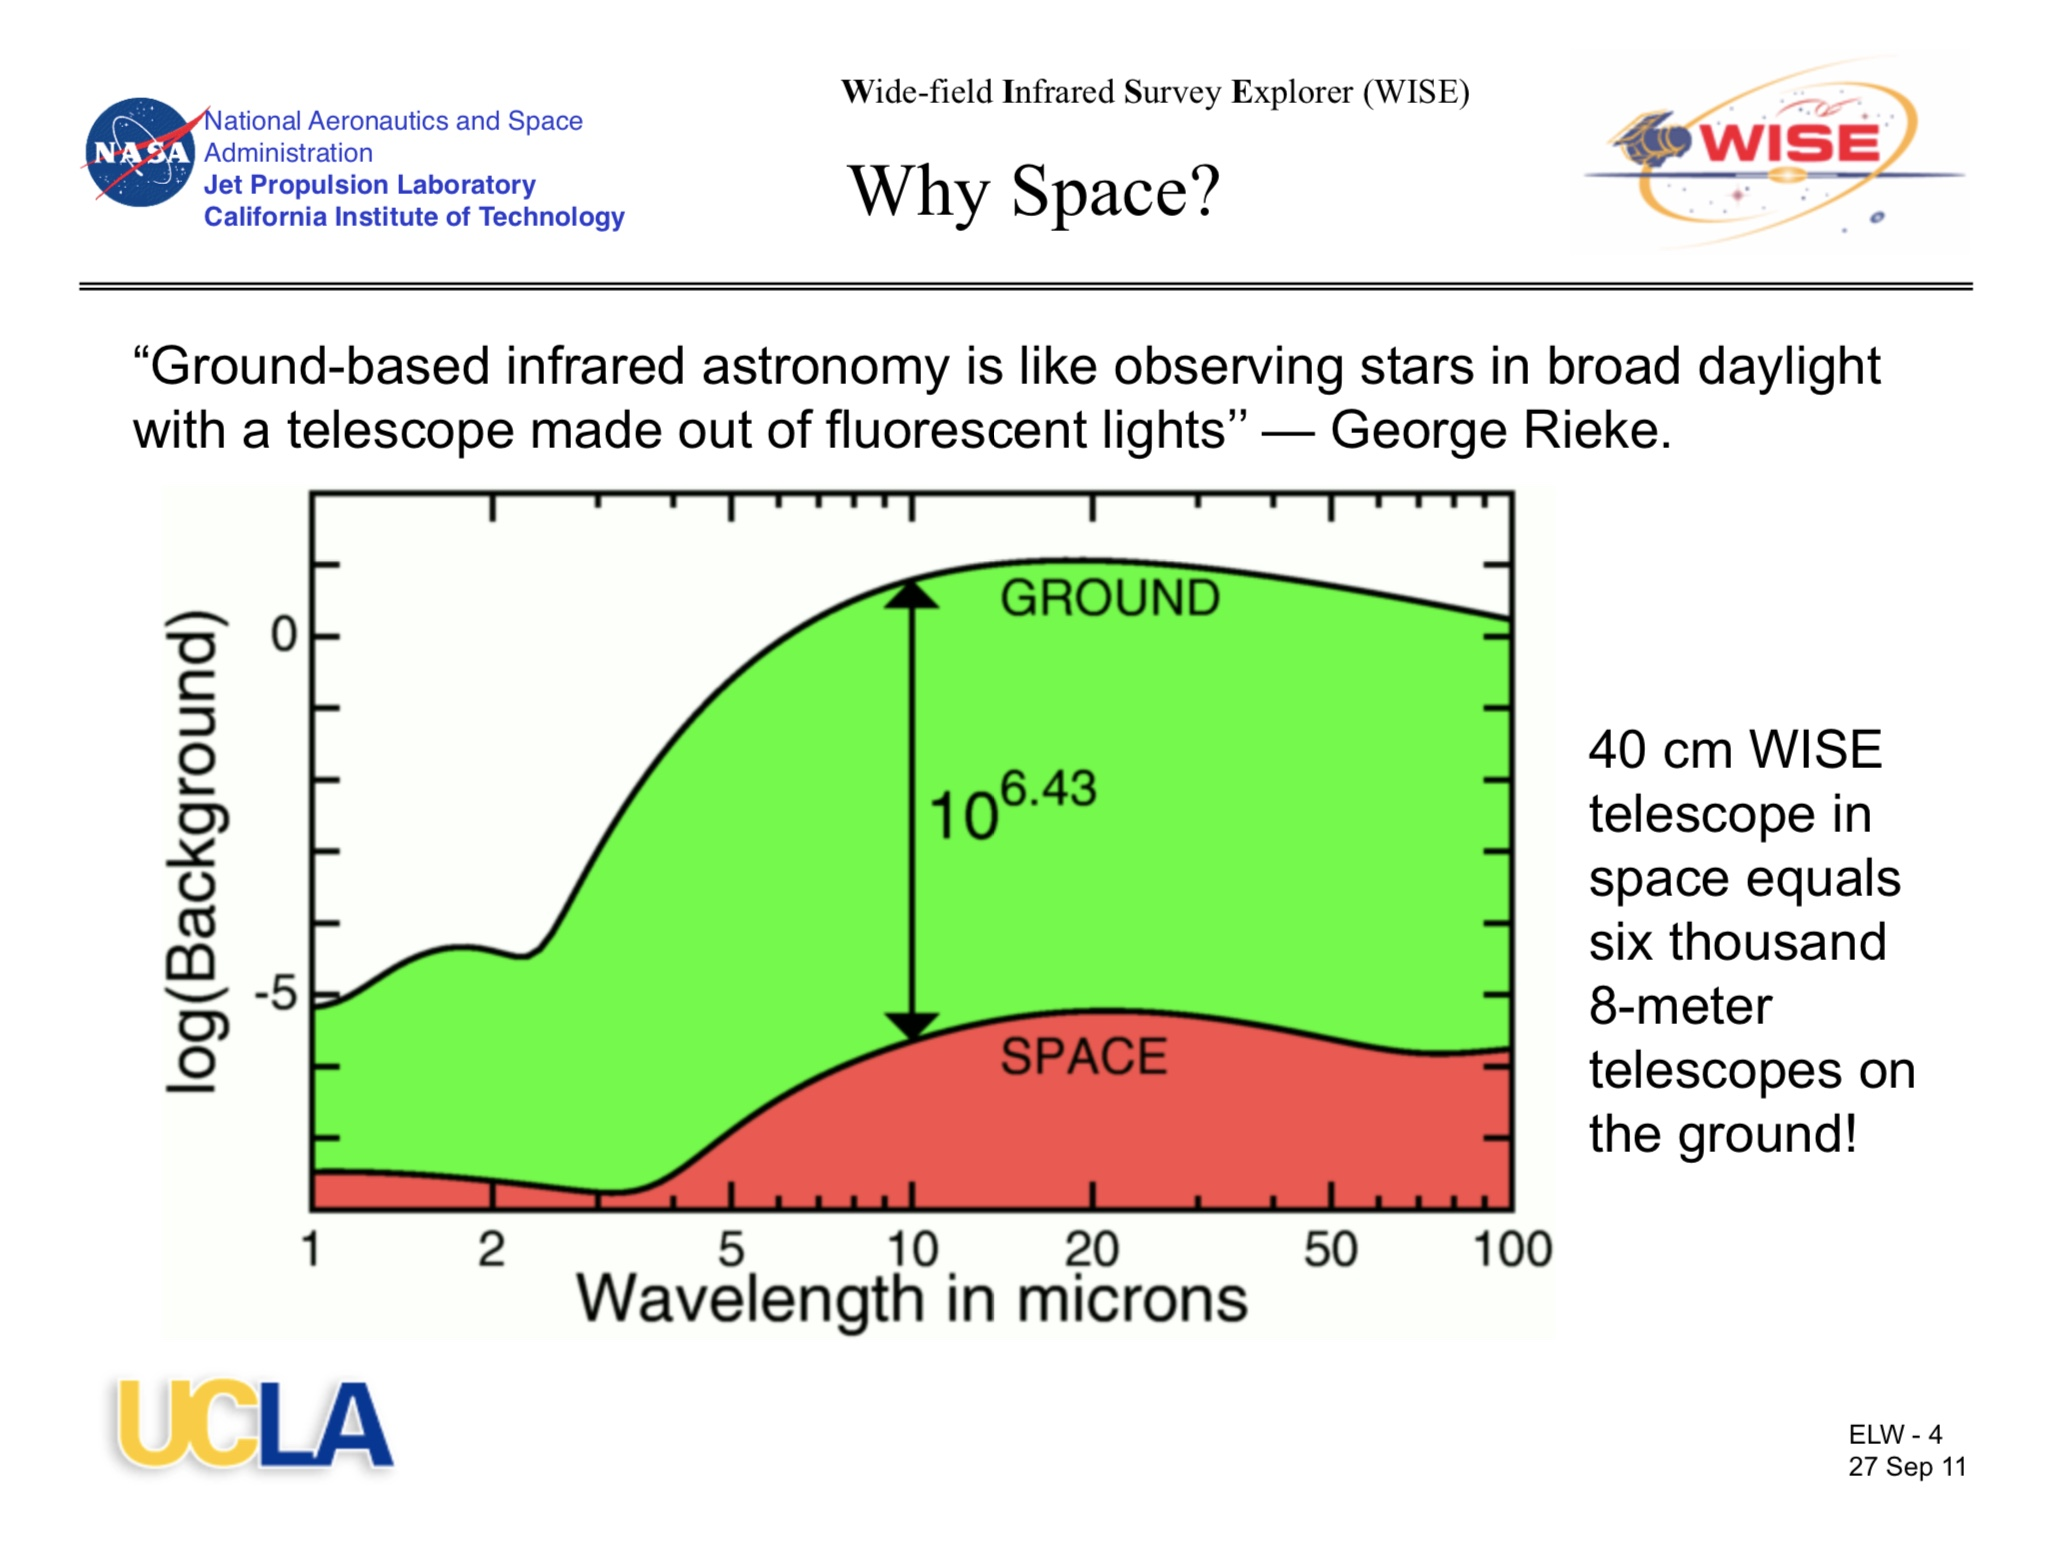
\includegraphics[height=12.0cm,width=16.0cm]{IR_Ground_vs_Space_backgrounds.jpeg}
    \vspace{-10pt}
\caption{Ned Wright's talk; 
https://www.ipac.caltech.edu/exgal2011/sched.shtml}
    \label{figtest-fig}
  \end{center}
\end{figure}

